\documentclass[../main.tex]{subfiles}

\begin{document}

GitLab part of the pipeline is built from 2 phases:
\begin{enumerate}
    \item \textbf{Building and pushing OCI images}\\
    Both \textit{reqour} and \textit{reqour-adjuster} images are built (using (among others) the corresponding JAR from Jenkins part). Once built, they are pushed to \url{https://quay.io/} image repository.
    \item \textbf{Deploying reqour}\\
    All PNC microservices run in OpenShift cluster. Helm is used for templating OpenShift resource files, which allow us to define a resource to all environments in a single file and replacing the values for corresponding environment when creating the chart.

    Created charts are stored in Helm PNC repository. Once the chart is successfully pushed to the repository, it is installed into the OpenShift cluster. OpenShift updates those resources which were affected by the current pipeline run, hence finishing the deployment.
\end{enumerate}

The above description is visualized in Figure \ref{fig:gitlab}.

\begin{figure}
  \begin{center}
    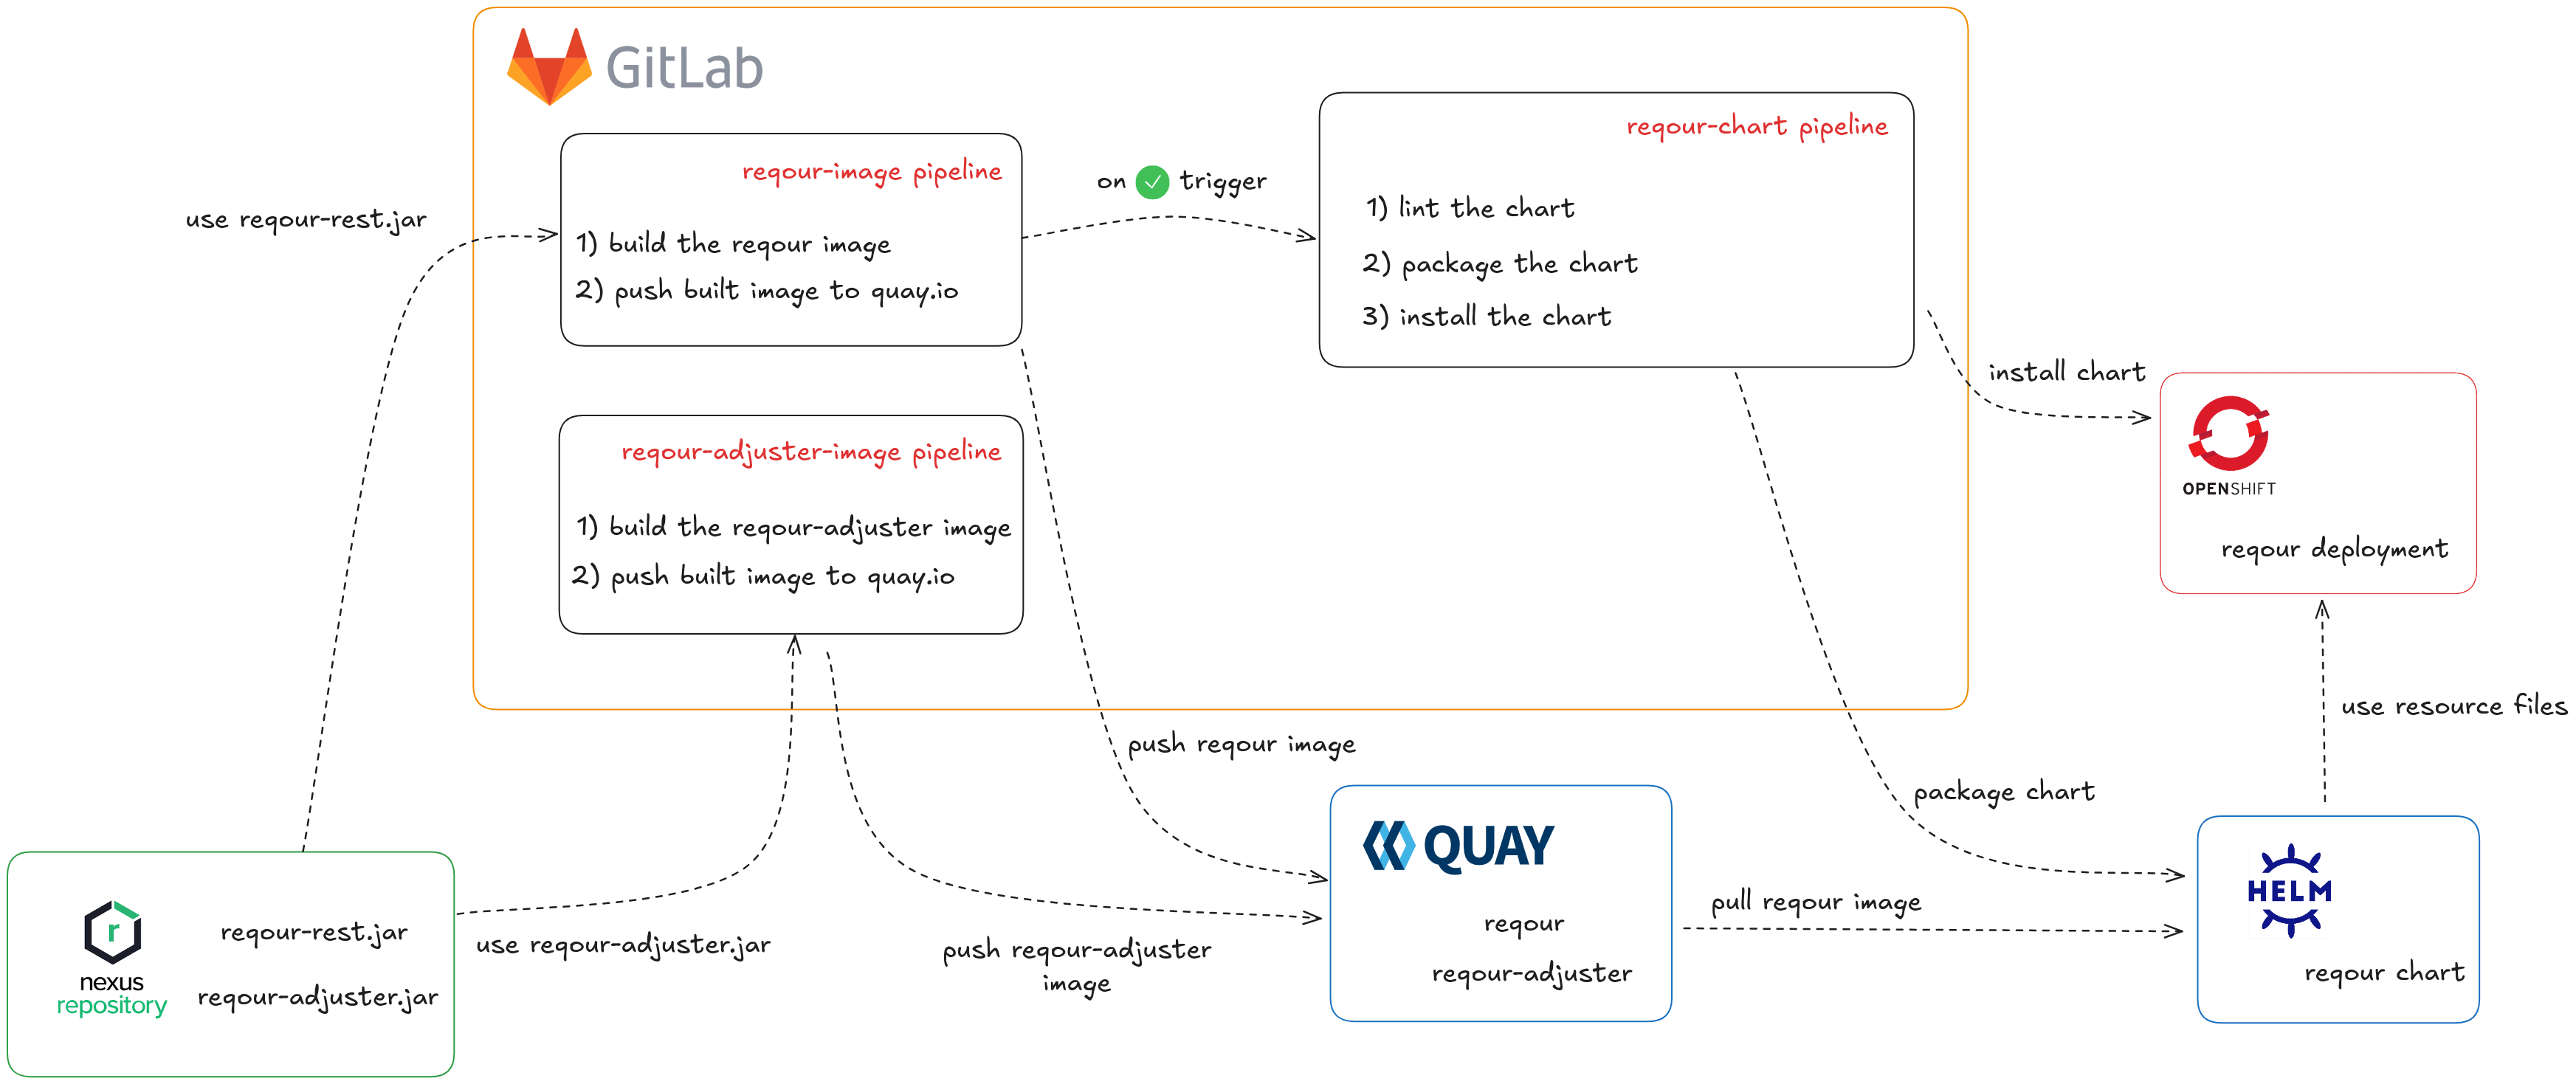
\includegraphics[width=\textwidth]{images/gitlab.png}
  \end{center}
  \caption{GitLab part of the pipeline}
  \label{fig:gitlab}
\end{figure}

\end{document}
